% https://www.baeldung.com/cs/sliding-window-algorithm
\section{Codeforces 676C: Vasya and String}
\begin{itemize}
    \item Problem link: \url{https://codeforces.com/contest/676/problem/C}
    \item Here, we learn how to write a proof of correctness for sliding window where the window length is \emph{upper bounded}. That is,
        we have a \emph{maximum} length of sliding window that we cannot exceed.
    \item \emph{Key Idea 1}: consider all windows that contain legal solutions. Suppose we have two windows $[l_1, r_1]$ and $[l_2, r_2]$
        where $r_1 < r_2$ (that is, window $1$ ends before window $2$). Then, we wish to show that $l_1 < l_2$ (that is, window $1$
        begins before window $2$).
    \item This condition implies that when we make progress by moving $r_1 \rightarrow r_2$, we can similarly make forward progress
      moving $l_1 \rightarrow l_2$. We would not have to go backwards, like
      $l_2 \leftarrow l_1$.  So when we move from $r$ to $(r+1)$, we need to
      decide how much we must move $l$. We know that this will not lose
      solutions from the prior invariant.
\end{itemize}


Let's consider a simpler subproblem, where are given a string of \texttt{'a'}s and \texttt{'b'}s and we must find
the longest substring with at most $k$ \texttt{'b'}s. The original problem can be solved by solving this problem twice,
once with \texttt{'a, b'} and once by swapping these letters.

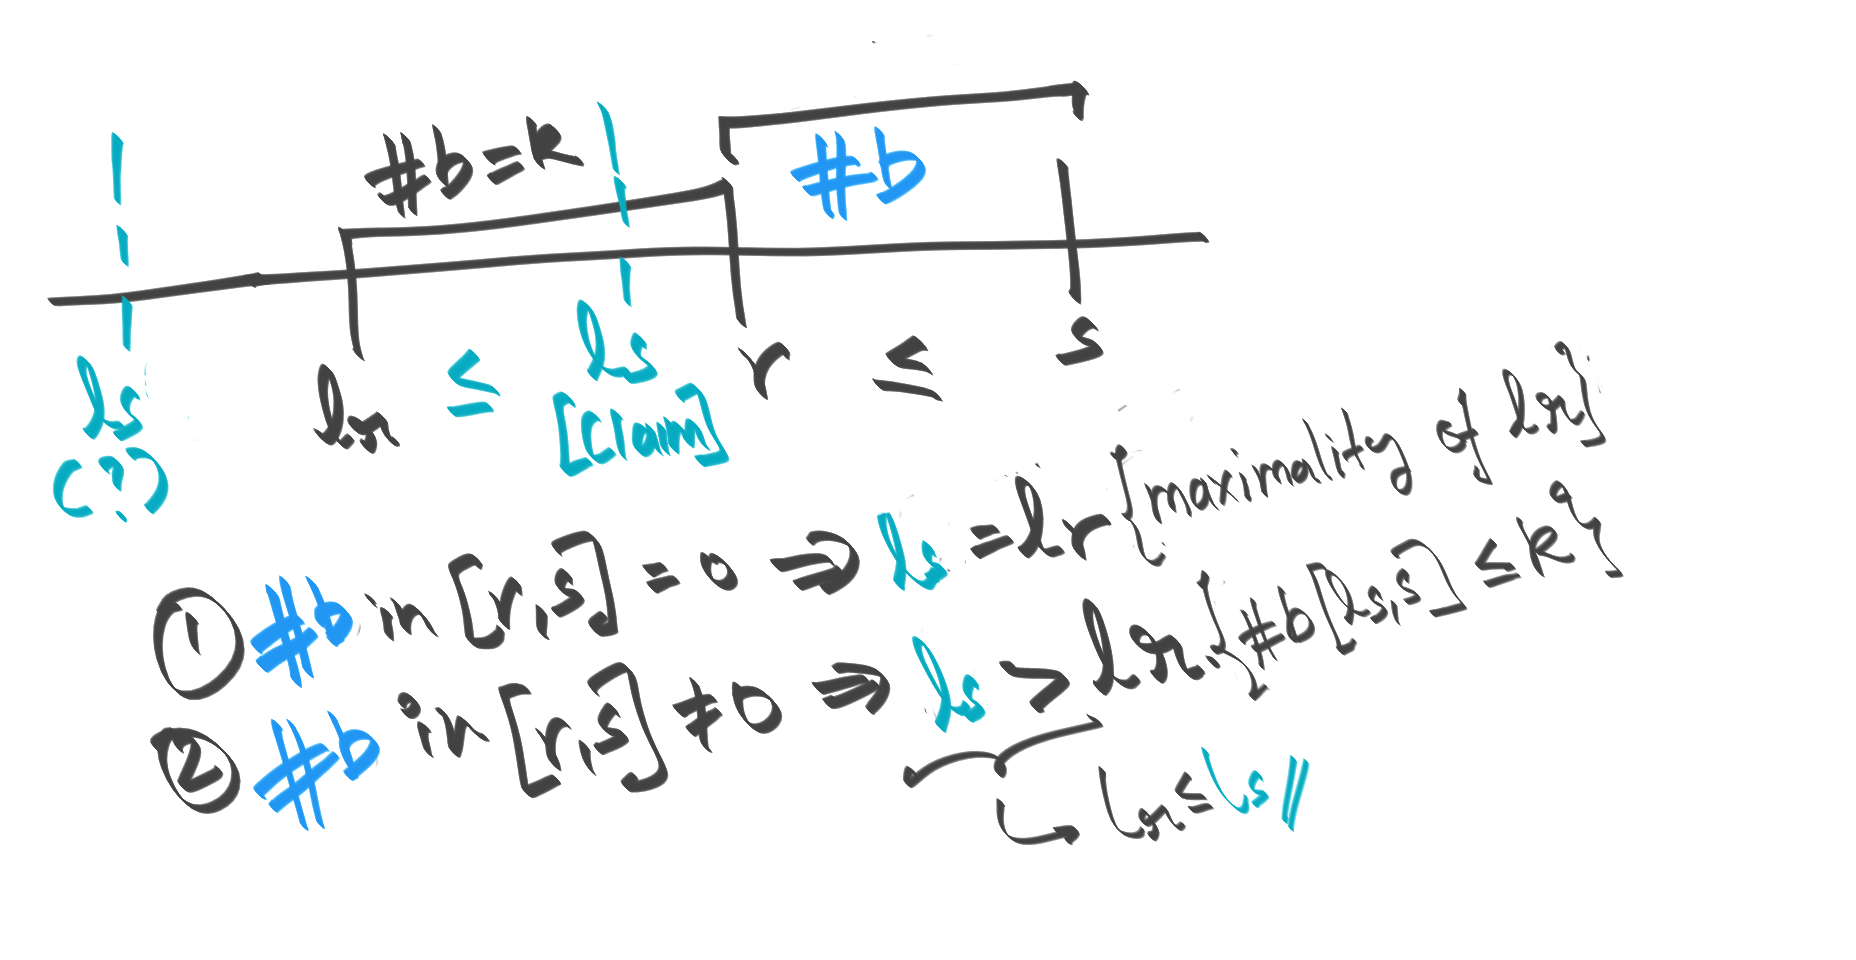
\includegraphics[width=\textwidth]{problems/676c/sliding-window-optimality.png}

\begin{itemize}
    \item At this subproblem, let us have $r \leq s$. We wish to show that $l_r \leq l_s$, where $l_x$ 
        is the leftmost index such that $[l_x \dots x]$ is a legal index. We begin by case analysis on the number of \texttt{'b'}s
        in the interval $[r, s]$.
    \item (a) zero \texttt{'b'}s in $[r, s]$: Then we claim that $l_s \geq l_r$ (In fact, $l_s = l_r)$. Suppose $l_s < l_r$.
        This means that the interval $[l_s < l_r \leq r \leq s]$ contains at most $k$ \texttt{'b'}s. Thus, the interval $[l_s < \l_r \leq r]$
        also contains at most $k$ \texttt{'b'}s. But this contradicts the maximality of the value $l_r$. Hence, $l_s \geq l_r$.
        This implies that $r \leq s \implies l_r \leq l_s$.
    \item (b) one or more \texttt{'b'}s in $[r, s]$. Then we claim that $l_s > l_r$. Suppose $l_s \leq l_r$.
        Since $l_r$ was maximal, we have either (b1) The interval $[l_r \dots r]$ has $k$ \texttt{'b'}s ($\# b(s[l_r, \dots, r]) = k$)
        or (b2) $l_r$ is the leftmost index ($l_r = 1$ and $\# b(s[l_r, \dots, r] < k$).
        \begin{itemize}
            \item (b1) in this case, we must have $l_s \geq l_r$. Suppose not. Then we have that $l_s < l_r < r < s$. So the interval
                $[l_r, r]$ is strictly contained in $[l_s, r]$ (which is also a legal interval). This contradicts the maximality of $l_r$.
            \item (b2) $l_r$ is the leftmost index possible, so we trivially have $l_r \leq l_s$.
        \end{itemize}
\end{itemize}

\begin{minted}{cpp}
// https://codeforces.com/contest/676/submission/121164663
void main() {
  ...
  int best = 0;
  for (int c = 'a'; c <= 'b'; ++c) {
    int l = 0;
    int changed = 0;
    // [l, r]
    for (int r = 0; r < n; ++r) {
      // change to c
      if (s[r] != c) { changed++; }
      while (changed > k) {
          if (s[l] != c) { changed--; }
          l++;
      }
      best = max(best, r - l + 1);
    }
  }
  cout << best;
}
\end{minted}


